\section{Результаты}\label{sec:results}
Стоит отметить, что в настоящее время метод SPSA играет ключевую роль в оптимизации; мы провели
серию экспериментов.
Момент -- в отличие от классической схемы -- сглаживает траекторию.
Метод не просто ускоряет сходимость, а делает её устойчивой к шуму --- это главный результат.
	Средняя ошибка после 300 итераций показана на рисунке.
\begin{equation}
E
=
\frac{1}{N}
\sum_i
\|x_i\|^2
\end{equation}
\begin{figure}[t]
\centering
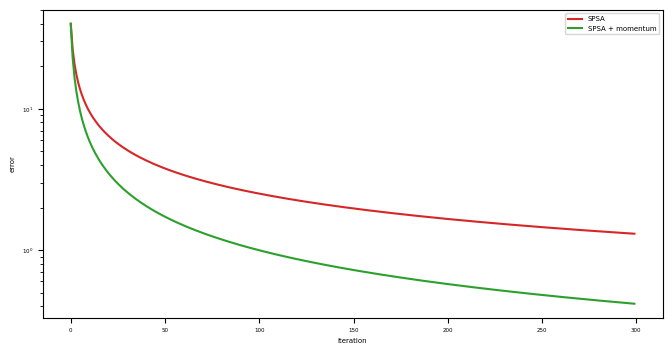
\includegraphics[width=\linewidth]{convergence_bad.png}
\caption{Сходимость SPSA и SPSA с моментом.}
\end{figure}
